To test the model, a cable with a pressure sensor has been put on the boat in order to capture the behaviour of the cable.



\section*{Boat specification}

The boat is a retrofitted version of the model Mini-12 and can be consider of the 2.4mR-class by the International Sailing Federation meaning is length is around 4 meters. It weigh around 300 kg.

To proceed to the measurement of the cable depth, a pressure sensor has been added and also an Arduino  Uno as  Analog to digital converter and send the sensor data to the computing unit a Raspberry Pi 3 Model B.

\begin{figure}[H]
\centering
    \begin{minipage}[b]{0.4\textwidth}
    \centering
    \includegraphics[scale=0.024,angle=0]{pressure_sensor.jpg}
    \caption{Pressure Sensor used to measure the depth of the cable.}
    \label{fig:pressure_sensor}
    \end{minipage}
    \hfill
    \begin{minipage}[b]{0.45\textwidth}
    \centering
    \includegraphics[scale=0.4,angle=0]{arduino_uno.jpg}
    \caption{Arduino Uno as a converter for the pressure sensor.}
    \label{fig:arduino_uno}
    \end{minipage}
\end{figure}

The data was first received be an xBee, a radio transmitter, and logged on a remote computer via Labview, but the data transfer was not reliable enough to get good interpretation of the results. Then the pressure sensor have been incorporated in the database (remote and local) , data is sent live to a web server to be saved and displayed via a 4G modem.

\begin{figure}[H]
\centering
    \begin{minipage}[b]{0.4\textwidth}
    \centering
    \includegraphics[scale=0.15,angle=0]{4Grouting.jpg}
    \caption{4G Hotspot sending data to the web server.}
    \label{fig:4grouting}
    \end{minipage}
    \hfill
    \begin{minipage}[b]{0.45\textwidth}
    \centering
    \includegraphics[scale=0.22,angle=0]{raspeberry.jpg}
    \caption{Raspeberry V3 Computing Unit of the sailboat.}
    \label{fig:raspeberry}
    \end{minipage}
\end{figure}

The Raspberry Pi is running Arch Linux and the program controlling the boat is written in C++ (see~\ref{sec:simulator} for more details).

\section{Test process}

First the gathered data will be compared with the old model to see if the new one add any advantage in the design of controller.It is not certain to see a lot a differences between the similarity of each model of the boat to the real test, as said before the model does not take into account the roll of the boat , this can change the expected value of the pressure sensor.

 The goal is to determine is the simulation of the cable is usable and to see if the new model of the boat will be useful in the conception of new controller handling the cable. 
 
 The test procedure is quite simple
 
\begin{itemize}
\item Cable added on the hull of the boat (between 6 and 20 m) with a linear mass of 130 g/m
\item Tapping a pressure sensor on the cable, the length of the cable attached to the pressure sensor is 6 meters
\item Boat has to reach multiple waypoints while measuring the depth of the pressure sensor
\item Boat redo the same path without cable
\end{itemize}

As the pressure sensor cable is smaller than the long one (3 meters in the water), to compare to the simulation, we take the values of the depth of the cable in the simulation at 3 meters length.


\begin{figure}[H]
\centering
    \begin{minipage}[b]{0.4\textwidth}
    \centering
    \includegraphics[width=5cm,angle=0]{launching_boat.jpg}
    \caption{Lowering the boat in the water.}
    \label{fig:lowerboat}
    \end{minipage}
    \hfill
    \begin{minipage}[b]{0.45\textwidth}
    \centering
    \includegraphics[width=5cm,angle=0]{sailingrobot.jpg}
    \caption{Sailbot sailing during a test.}
    \label{fig:sailbot_test}
    \end{minipage}
\end{figure}

\section{Validation of cable simulation}

First the depth of the pressure sensor will be compared to the depth of the simulation of the cable when taking the speed and position data.

\begin{figure}[H]
\centering
    \begin{minipage}[b]{0.4\textwidth}
    \centering
    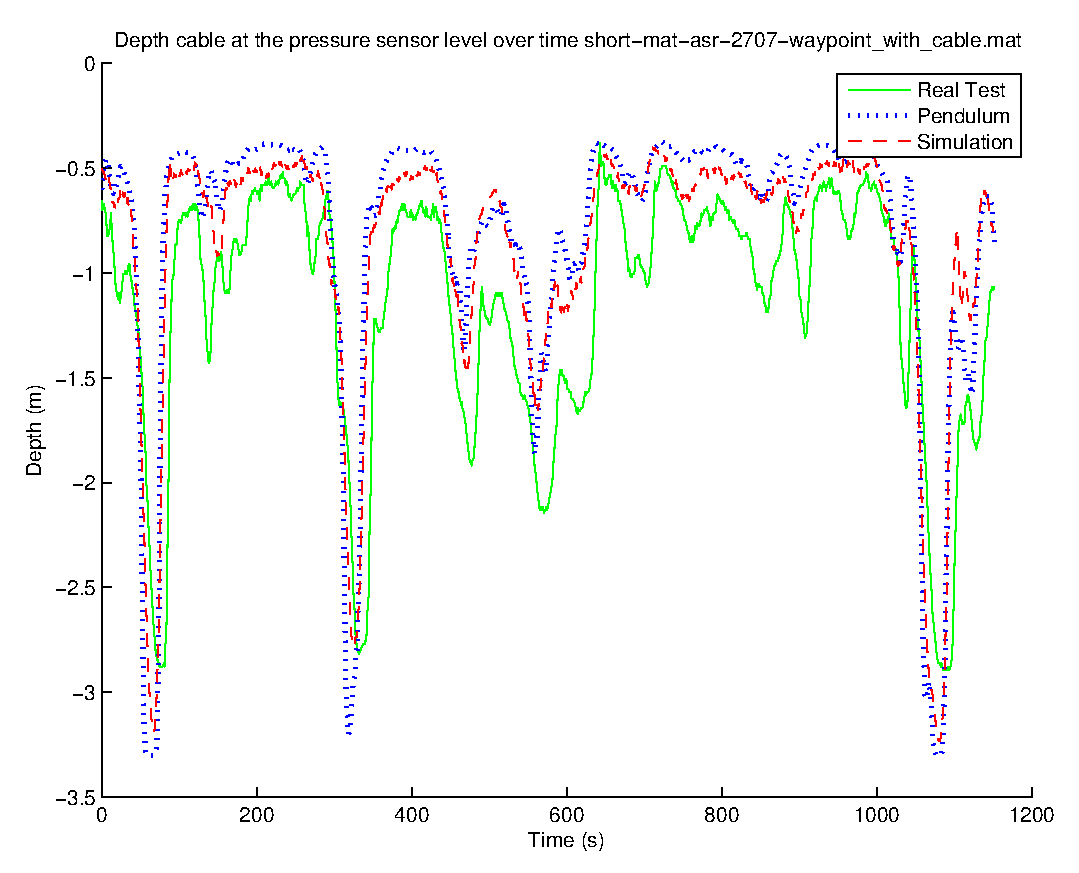
\includegraphics[scale=0.4,angle=0]{depth_time_2707}
    \caption{Comparison between depth of cable at the pressure sensor level in simulation and real test.}
    \label{fig:comp_depth_time_2007}
    \end{minipage}
    \hfill
    \begin{minipage}[b]{0.45\textwidth}
    \centering
    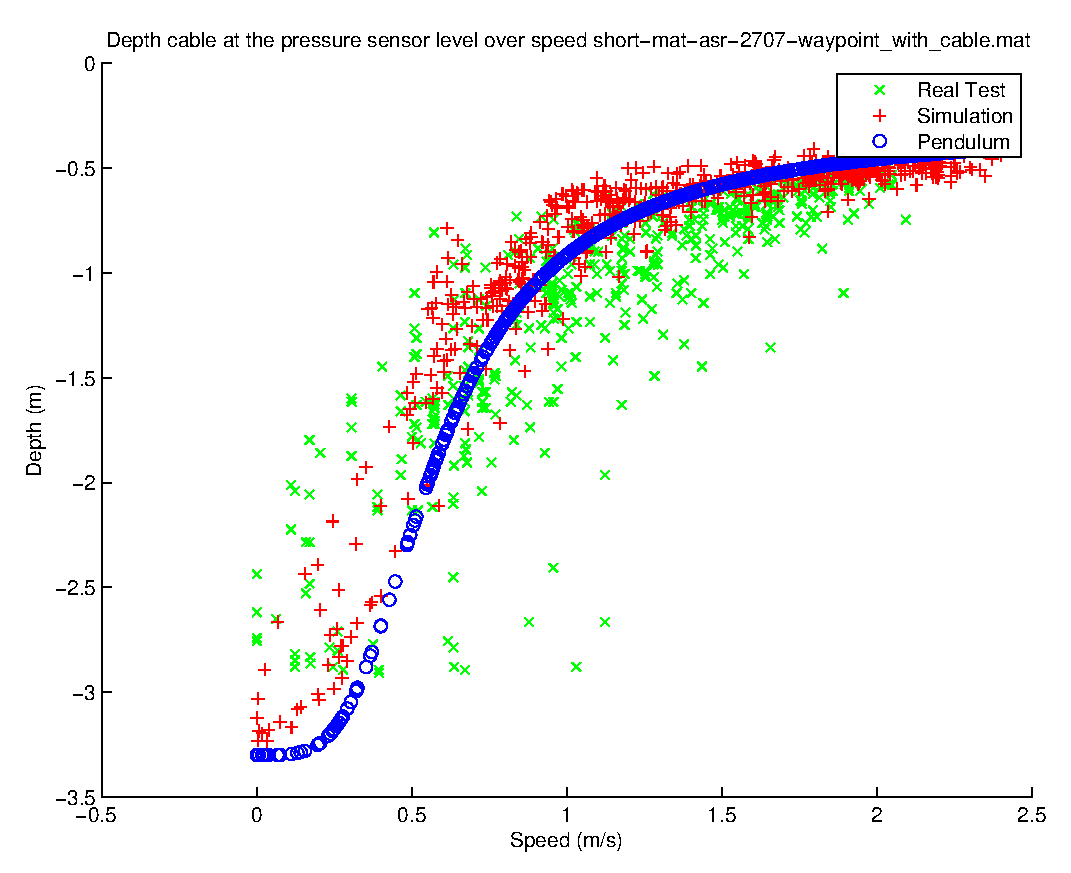
\includegraphics[scale=0.4,angle=0]{depth_speed_2707}
    \caption{Comparison of depth of cable at the pressure sensor level in function of speed between simulation and real test.}
    \label{fig:comp_depth_speed_2007}
    \end{minipage}
\end{figure}

To simulate the run of the boat with the simulation of the cable , the \gls{GPS} position data from the run is taken and filtered, and then feed to the simulator, the cable consider the positions as a fixed point of the cable.

The figure~\ref{fig:comp_depth_time_2007} hold three profile of depth, the real test, the depth computed by simulation and one computed with the formula from~\ref{equ_theta_1}. The first conclusion is that the depth of the cable in the test is similar to the simulation and the profile from the pendulum model too.
 In the same way the profile of depth over speed is also close between test and simulation.
 
 The simulation has an mean offset off 34 cm and the pendulum  43 cm so if we consider the simulation close enough we can consider also the pendulum to be close enough as way to predict the depth of the cable at a certain speed.
 
 \begin{figure}[H]
\centering
    \begin{minipage}[b]{0.4\textwidth}
    \centering
    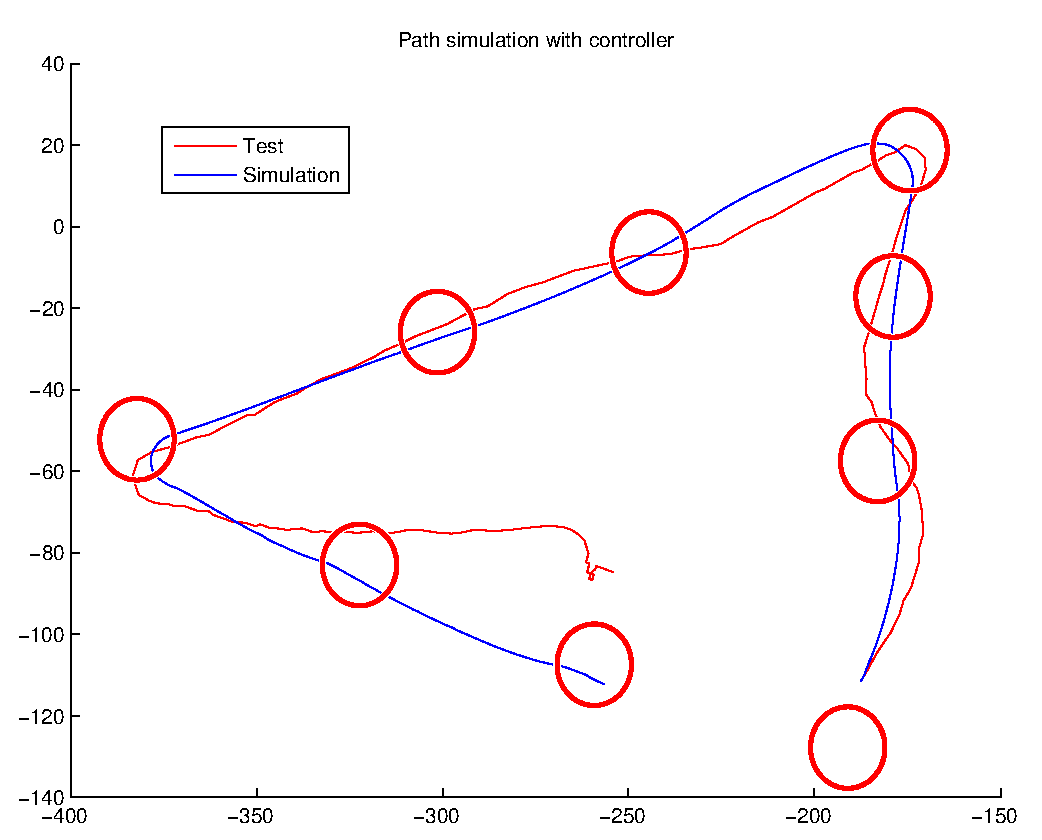
\includegraphics[scale=0.4,angle=0]{simulation_path_controller_with_cable_3006}
    \caption{Comparison of path between simulation and test with cable 416 s.}
    \label{fig:comp_w_cable_3006}
    \end{minipage}
    \hfill
    \begin{minipage}[b]{0.45\textwidth}
    \centering
    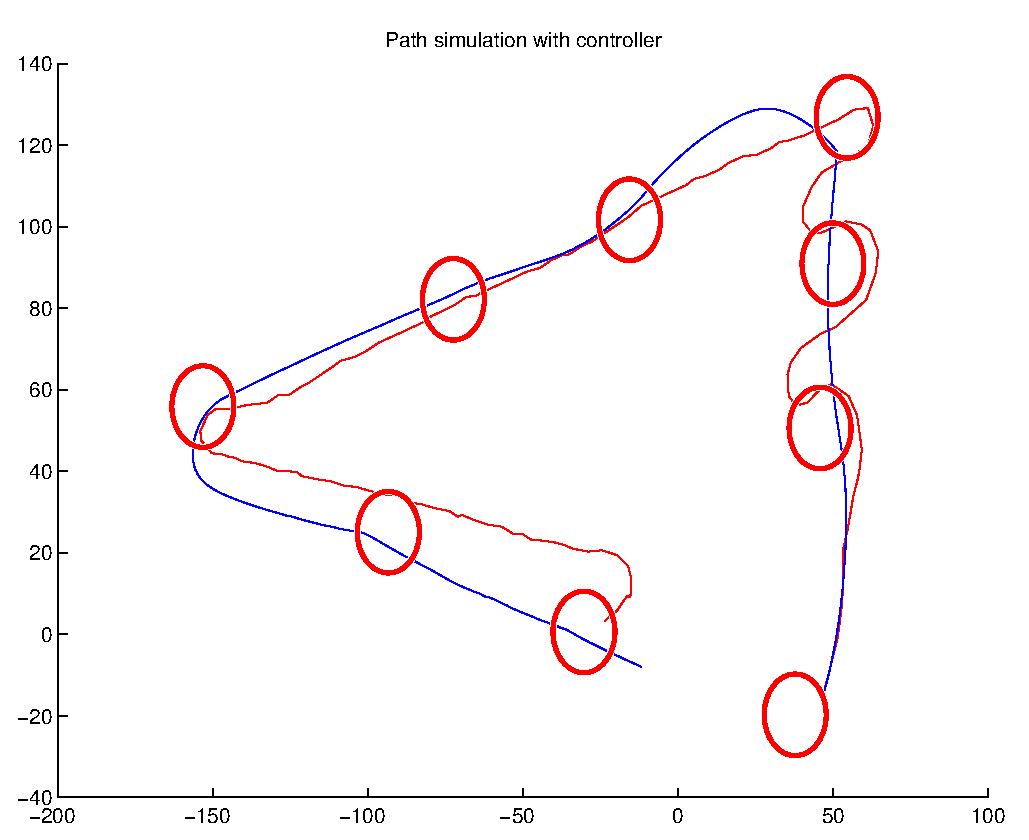
\includegraphics[scale=0.4,angle=0]{simulation_path_controller_without_cable_3006}
    \caption{Comparison of path between simulation and test without cable 430 s.}
    \label{fig:comp_wt_cable_3006}
    \end{minipage}
\end{figure}

In the simulation runs represented in~\ref{fig:comp_w_cable_3006} and~\ref{fig:comp_wt_cable_3006} the simulation follow the same algorithm that the one on the boat.

 \begin{figure}[H]
    \centering
    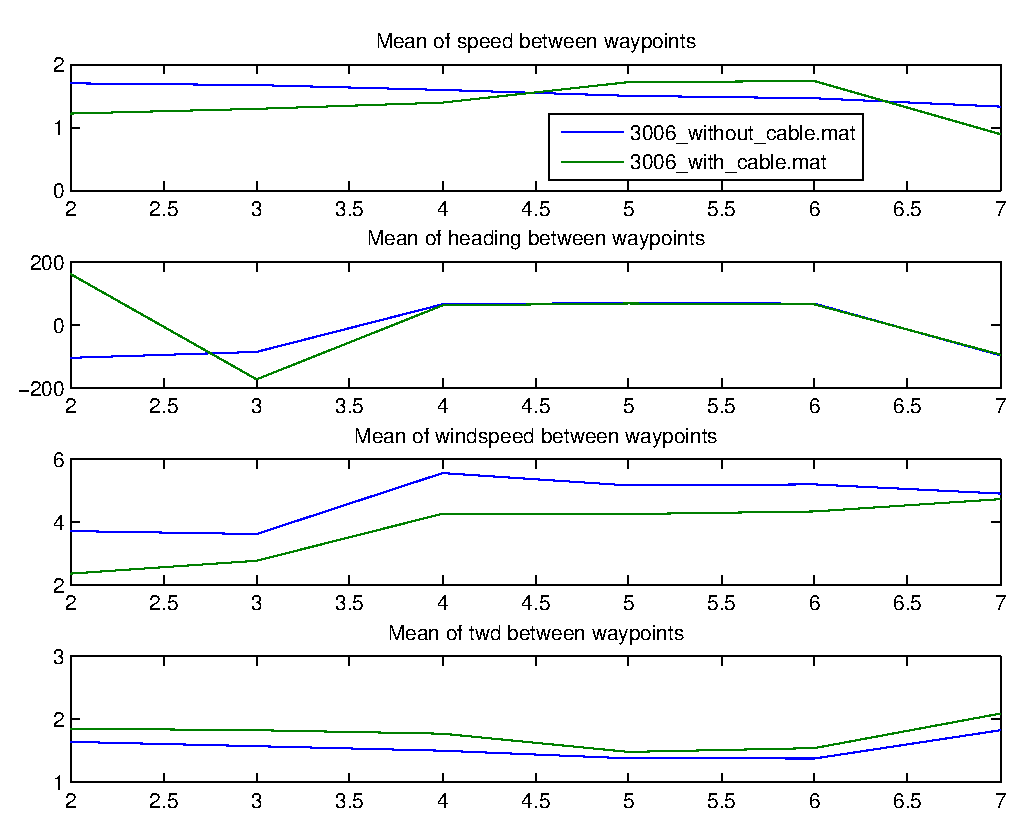
\includegraphics[scale=0.4,angle=0]{comp_run_test_3006}
    \caption{Comparison of some significant values between waypoints for the test.}
    \label{fig:comp_run_306}
\end{figure}

The figure ~\ref{fig:comp_w_cable_3006} compare the speed,heading of the boat and the direction and speed of the wind between a run with the cable and a run without it. The most interesting part is between the waypoints 4 and 7 ( the value at 4 represent the mean value between the waypoints 4 and 5)  because the boat have the same mean heading. At the point 4 the speed of the boat without cable is greater than the speed of the boat without cable however the wind speed is also bigger than the run without cable so we can't conclude that the cable slow down the boat. And at the point 6 the situation is quite odd as the speed of the boat with cable is faster 
even though the wind speed during its run is smaller.

When considering the path of the boat during the simulations runs it is really similar and may change only because of the wind effect.

Considering this it can be supposed that the cable has a little effect on the boat and even in the simulation the differences are not big enough to make the design of a controller require its own model, as long as the cable remains relatively lightweight.
	



 